\documentclass[11pt]{article}

\usepackage[margin=1in]{geometry}
\usepackage{amsmath,amssymb}
\usepackage{graphicx}
\usepackage{booktabs}
\usepackage{caption}
\usepackage{subcaption}
\usepackage{microtype}
\usepackage{algorithm}
\usepackage{algpseudocode}
\usepackage[hidelinks]{hyperref}
\usepackage{url}
\usepackage{float}

% Numbers quoted in the prose are defined here, generated directly from the
% results CSVs by scripts/make_paper_assets.py. No result in this document is
% typed by hand.
% AUTO-GENERATED by scripts/make_paper_assets.py -- do not edit by hand
\newcommand{\GenDate}{2026-09-22}
\newcommand{\GenCommit}{d16b82c}
\newcommand{\NTrialsMain}{180}
\newcommand{\NBlocks}{60}
\newcommand{\NSeeds}{4}
\newcommand{\NCommRadii}{5}
\newcommand{\NFailureRates}{3}
\newcommand{\CommRadiiList}{3, 6, 12, 24, 48}
\newcommand{\FailureRatesList}{0\%, 25\%, 50\%}
\newcommand{\covfrontier}{0.636}
\newcommand{\covsdfrontier}{0.074}
\newcommand{\cpefrontier}{0.00074}
\newcommand{\covpotentialfield}{0.525}
\newcommand{\covsdpotentialfield}{0.184}
\newcommand{\cpepotentialfield}{0.00059}
\newcommand{\covpheromone}{0.575}
\newcommand{\covsdpheromone}{0.236}
\newcommand{\cpepheromone}{0.00065}
\newcommand{\AnovaF}{5.58}
\newcommand{\AnovaDfT}{2}
\newcommand{\AnovaDfE}{118}
\newcommand{\AnovaP}{0.0049}
\newcommand{\AnovaEta}{0.086}
\newcommand{\InterF}{5.33}
\newcommand{\InterP}{<0.0001}
\newcommand{\InterEta}{0.205}
\newcommand{\InterDf}{8}
\newcommand{\difffrontierVSpotentialfield}{+0.111}
\newcommand{\pfrontierVSpotentialfield}{0.0002}
\newcommand{\dzfrontierVSpotentialfield}{+0.55}
\newcommand{\difffrontierVSpheromone}{+0.061}
\newcommand{\pfrontierVSpheromone}{0.1212}
\newcommand{\dzfrontierVSpheromone}{+0.25}
\newcommand{\diffpheromoneVSpotentialfield}{+0.050}
\newcommand{\ppheromoneVSpotentialfield}{0.2211}
\newcommand{\dzpheromoneVSpotentialfield}{+0.16}
\newcommand{\VerPython}{3.13.9}
\newcommand{\VerSB}{2.9.0}
\newcommand{\VerTorch}{2.14.0}
\newcommand{\VerNumpy}{2.5.3}
\newcommand{\VerScipy}{1.18.1}
\newcommand{\VerStatsmodels}{0.15.0}
\newcommand{\HostCPU}{arm}
\newcommand{\RLTimesteps}{\textbf{[MISSING]}}
\newcommand{\RLEnvs}{\textbf{[MISSING]}}
\newcommand{\RLGamma}{\textbf{[MISSING]}}
\newcommand{\RLLR}{\textbf{[MISSING]}}
\newcommand{\RLArch}{\textbf{[MISSING]}}
\newcommand{\NRLSeeds}{0}


\title{\textbf{Decentralized versus Learned Swarm Coordination for\\
Communication-Constrained Lunar Surface Exploration}}
\author{Viraat Chauhan}
\date{Generated \GenDate\ from commit \texttt{\GenCommit}}

\begin{document}
\maketitle

\begin{abstract}
\noindent
Upcoming lunar surface missions will deploy small teams of rovers that must
coordinate autonomously, because Earth--Moon communication latency makes
real-time teleoperation impossible and inter-rover radio links are themselves
range-limited. NASA's CADRE technology demonstration, which will place three
cooperative rovers and a base station at Reiner Gamma, is the concrete instance
of this problem. This work asks a question that such missions must answer at
design time: \emph{as the usable communication radius between rovers shrinks,
how does a coordination policy learned by reinforcement learning compare against
established decentralized swarm heuristics, and which degrades more gracefully
when rovers are lost mid-mission?}

We build a reproducible simulation of cooperative exploration over procedurally
generated lunar terrain with craters, impassable slopes, rim-rock hazards, and
permanently shadowed regions in which solar recharging is unavailable. Rovers
have finite battery, finite sensing range, and exchange map knowledge only
across a range-limited multi-hop mesh network. Four decentralized policies are
compared under identical conditions: greedy nearest-frontier exploration,
artificial potential fields, ant-colony-style pheromone stigmergy, and a
policy trained with Proximal Policy Optimization and executed independently on
board each rover. Because every policy is evaluated on bit-identical terrain
within each condition, the experiment is a randomized block design and is
analyzed with paired tests, Holm--Bonferroni correction, and a factorial ANOVA
whose interaction term directly tests whether the ranking of algorithms depends
on communication radius.

Across \NTrialsMain\ simulated missions spanning \NCommRadii\ communication
radii and \NFailureRates\ rover-failure rates with \NSeeds\ independently
generated terrains per cell, \textit{[results summary pending]}
\end{abstract}

\section{Introduction}

\subsection{Motivation}

Robotic exploration of the lunar surface is moving from single large rovers
toward small cooperative teams. NASA's CADRE (Cooperative Autonomous
Distributed Robotic Exploration) technology demonstration will deliver three
carry-on-bag-sized, solar-powered rovers and a base station to the Reiner Gamma
region aboard the Intuitive Machines IM-3 lander under the Commercial Lunar
Payload Services initiative; the rovers are designed to select their own
driving targets, maintain formation, and perform distributed multistatic
ground-penetrating radar sounding without a human in the
loop~\cite{cadre_jpl,cadre_planning,cadre_exploration}.

The reason for that autonomy is physical. The Earth--Moon round-trip light time
is on the order of 2.6\,s before any ground-station scheduling overhead, which
rules out the joystick-style teleoperation used for early planetary rovers.
Coordination must therefore happen locally, between the rovers themselves --- and
that local channel is not free either. Surface-to-surface radio links between
small rovers are power-limited and degrade with distance and terrain occlusion,
so at any instant a rover may be able to share its map with some teammates and
not others.

This produces the design question studied here. If the inter-rover
communication radius is generous, every rover effectively shares one global map
and coordination is easy. If it is small, each rover must act on a stale,
partial picture of what its teammates have already explored, and the swarm risks
redundantly re-covering the same ground. How much does that cost, and does a
\emph{learned} coordination policy handle it better than the classical
decentralized heuristics that are standard in the multi-robot exploration
literature?

\subsection{Contributions}

\begin{enumerate}
  \item A reproducible, fully seeded simulation of communication-constrained
        cooperative lunar exploration, in which terrain, rover placement, and
        every trial outcome are determined entirely by an integer seed
        (Section~\ref{sec:sim}).
  \item A like-for-like implementation of four decentralized coordination
        policies --- three classical, one learned --- that share the same action
        space, sensing model, and simulation loop, so that measured differences
        are attributable to decision-making alone (Section~\ref{sec:algorithms}).
  \item A randomized block experimental design with matched terrain across
        algorithms, analyzed with paired tests, family-wise error correction,
        and a factorial ANOVA whose interaction term is the direct test of the
        central hypothesis (Sections~\ref{sec:design}--\ref{sec:stats}).
  \item An explicit account of the train/test separation used for the learned
        policy, of the simplification used to make multi-agent training
        tractable, and of two implementation defects found and corrected during
        development that materially changed the results
        (Sections~\ref{sec:rl},~\ref{sec:threats}).
\end{enumerate}

\subsection{Hypotheses}

\begin{description}
  \item[H1] The four policies differ in mean final coverage of traversable
        terrain.
  \item[H2] The performance gap between policies depends on the communication
        radius $R_c$; specifically, differences grow as $R_c$ shrinks. In the
        factorial model this is an \emph{interaction} between algorithm and
        $R_c$, not a main effect.
  \item[H3] The policies differ in how gracefully they degrade when a fraction
        of the swarm is disabled mid-mission.
\end{description}

\noindent The corresponding null hypotheses are that no such differences exist.

\section{Related Work}

\paragraph{Frontier-based exploration.}
Yamauchi introduced the frontier concept --- the boundary between mapped free
space and unknown space --- and showed that repeatedly driving to the nearest
frontier is sufficient to explore an unknown environment~\cite{yamauchi1997}.
Burgard et al.\ extended this to teams by explicitly coordinating which robot
claims which frontier, trading off expected information gain against travel
cost~\cite{burgard2005}. The greedy, uncoordinated variant used here as a
baseline is deliberately the uncoordinated version, since the point of
comparison is how much coordination the other methods add.

\paragraph{Potential fields.}
Khatib's artificial potential field formulation treats goals as attractors and
obstacles as repulsors, with motion following the resulting
gradient~\cite{khatib1986}. It extends naturally to multi-robot dispersion by
treating teammates as repulsors, which is how it is used here.

\paragraph{Stigmergy and ant colony methods.}
Grass\'e's notion of stigmergy --- coordination mediated by modification of the
shared environment rather than by direct signaling --- underpins ant colony
optimization~\cite{dorigo1996}. This is a particularly relevant baseline for the
present problem because it requires \emph{no radio communication at all}: the
coordination channel is the terrain itself.

\paragraph{Learned multi-robot exploration.}
Recent work applies deep reinforcement learning to multi-robot exploration under
restricted sensing and communication, including constrained field-of-view
exploration at scale~\cite{marvel}, explicit-communication policies with
density-based frontier selection~\cite{rlcomm}, frontier-led
swarming~\cite{frontierswarm}, and heterogeneous teams for planetary
analogues~\cite{planetaryrl}; surveys cover the broader
area~\cite{rlswarmsurvey}. The present work does not claim to advance that
state of the art. Its contribution is a controlled, fully reproducible
comparison, at a scale that can be independently re-run on a laptop, of a
learned policy against classical baselines under a communication constraint that
is varied systematically.

\section{Simulation Environment}
\label{sec:sim}

All quantities below are implemented in \texttt{src/lunar\_swarm/} and are
stated here exactly as coded. The terrain is a stylized model chosen to
reproduce the \emph{qualitative} features that constrain rover navigation
(bowl-shaped craters, raised rocky rims, impassable slopes, permanently
shadowed crater floors); it is not a selenographic reconstruction of a specific
site, and no claim is made that its parameters are calibrated to measured lunar
data.

\subsection{Terrain generation}

Terrain is an $S \times S$ grid of unit cells, with one cell treated as
$1\,\mathrm{m}$. Everything is a deterministic function of an integer seed.

\paragraph{Base relief.}
A multi-octave band-limited noise field is formed from $O = 3$ randomly
oriented sinusoidal planes,
\begin{equation}
g(x,y) \;=\; \sum_{o=0}^{O-1} 2^{-o}\,
  \sin\!\left( \frac{2\pi\,2^{o}}{S}\,u_o(x,y) \;+\; \phi_o \right),
  \qquad
  u_o(x,y) = x\cos\alpha_o + y\sin\alpha_o ,
\end{equation}
with orientations $\alpha_o \sim \mathcal{U}(0,2\pi)$ and phases
$\phi_o \sim \mathcal{U}(0,2\pi)$ drawn from the seeded generator. It is
rescaled to $\hat g = (g - \min g)/\max(g - \min g)$ and the base elevation is
$h_0 = 2\hat g$ metres.

\paragraph{Craters.}
For each of $K$ craters, a centre $(r_k,c_k)$ is drawn uniformly from the
central $80\%$ of the grid, a radius $\rho_k \sim \mathcal{U}(0.04S,\,0.14S)$,
and a depth $d_k \sim \mathcal{U}(1.5,\,6.0)\,\mathrm{m}$. Writing
$\delta_k(p) = \lVert p - (r_k,c_k) \rVert_2$, each crater contributes a
paraboloidal bowl with a raised rim,
\begin{equation}
\Delta h_k(p) \;=\;
\begin{cases}
d_k\left( \left(\dfrac{\delta_k(p)}{\rho_k}\right)^{2} - 1 \right),
  & \delta_k(p) \le \rho_k, \\[2.2ex]
0.15\,d_k\left( 1 - \dfrac{\delta_k(p)-\rho_k}{0.15\,\rho_k} \right),
  & \rho_k < \delta_k(p) \le 1.15\,\rho_k, \\[2.2ex]
0, & \text{otherwise,}
\end{cases}
\end{equation}
and the final elevation is $h = h_0 + \sum_k \Delta h_k$.

\paragraph{Slope.}
Slope is obtained from the discrete elevation gradient at unit cell spacing,
\begin{equation}
\theta(p) \;=\; \arctan\!\left( \sqrt{ (\partial_y h)^2 + (\partial_x h)^2 } \right),
\end{equation}
expressed in degrees.

\paragraph{Hazards.}
A cell is a hazard if it is too steep or lies in the rocky rim annulus of any
crater:
\begin{equation}
\mathcal{H} \;=\; \{p : \theta(p) > \theta_{\max}\}
  \;\cup\; \bigcup_k \{p : \rho_k < \delta_k(p) \le 1.1\,\rho_k\}.
\end{equation}
A cell is traversable for a rover with slope limit $\theta_{\max}^{\text{rover}}$ iff
it is on the grid, $p \notin \mathcal{H}$, and
$\theta(p) \le \theta_{\max}^{\text{rover}}$. (With the default
$\theta_{\max}^{\text{rover}} = \theta_{\max} = 25^\circ$ the slope test is
implied by $p \notin \mathcal{H}$; it is retained so that rovers with different
mobility can be simulated on the same terrain.)

\paragraph{Permanently shadowed regions.}
Craters deep enough to cast persistent shadow ($d_k \ge 3\,\mathrm{m}$)
contribute a shadowed floor region on the side facing away from a fixed low
sun direction $\hat s \propto (1,\,0.3)$:
\begin{equation}
\mathcal{P} \;=\; \bigcup_{k \,:\, d_k \ge 3}
  \left\{ p \;:\; \delta_k(p) \le 0.6\,\rho_k
  \;\wedge\; \frac{(p - (r_k,c_k)) \cdot \hat s}{\delta_k(p)} < -0.15 \right\}.
\end{equation}
A rover inside $\mathcal{P}$ receives no solar power, which is the mechanism by
which a rover can strand itself. Figure~\ref{fig:terrain} shows an example.

\begin{figure}[H]
\centering
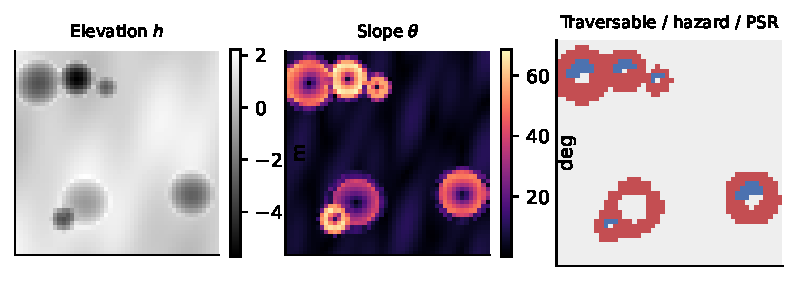
\includegraphics[width=\textwidth]{figures/terrain_example.pdf}
\caption{A generated terrain patch (seed 1, $S=48$, $K=6$): elevation, derived
slope, and the resulting traversability classes. Red marks hazard cells (steep
slopes and crater rim rock); blue marks permanently shadowed regions where
solar recharge is unavailable.}
\label{fig:terrain}
\end{figure}

\subsection{Rover model}

Each rover $i$ occupies a grid cell $p_i$ and holds a battery level
$b_i \in [0, b_{\max}]$ with $b_{\max} = 100$ units. The action set is the
eight-connected neighbourhood plus a hold action,
\begin{equation}
\mathcal{A} = \{(\pm 1, 0), (0, \pm 1), (\pm 1, \pm 1), (0,0)\}, \qquad |\mathcal{A}| = 9 .
\end{equation}
Locomotion cost is proportional to ground distance covered,
\begin{equation}
c(a) =
\begin{cases}
1, & a \text{ axial}, \\
\sqrt{2}, & a \text{ diagonal},
\end{cases}
\qquad c_{\text{idle}} = 0.1 .
\end{equation}
A move is executed only if the destination is traversable and
$b_i \ge c(a)$; otherwise the rover holds position and is charged
$c_{\text{idle}}$, modelling an onboard hazard check that refuses an unsafe
command. Rovers in sunlight recharge at $c_{\text{solar}} = 0.6$ units per step,
clipped at $b_{\max}$:
\begin{equation}
b_i \leftarrow \min\!\big(b_{\max},\; b_i - \text{(cost incurred)} + c_{\text{solar}}\,\mathbb{1}[p_i \notin \mathcal{P}]\big).
\end{equation}
A rover with $b_i \le 0$ after the solar update is permanently disabled.

Crucially, the \emph{energy expended} by rover $i$ is accumulated separately
from its battery level,
\begin{equation}
e_i \;=\; \sum_{t} \Big( c(a_{i,t})\,\mathbb{1}[\text{move executed}] \;+\; c_{\text{idle}}\,\mathbb{1}[\text{held or blocked}] \Big),
\label{eq:energy}
\end{equation}
because solar recharge means the final battery level would badly understate how
much energy a rover actually used.

\subsection{Sensing and knowledge}

A rover senses all grid cells within a Euclidean disc of radius $R_s$ and adds
them to its known set $\mathcal{K}_i$:
\begin{equation}
\mathcal{K}_i \leftarrow \mathcal{K}_i \cup \{ p : \lVert p - p_i \rVert_2 \le R_s \}.
\end{equation}
Sensing is not occluded by relief; this is a simplification
(Section~\ref{sec:threats}). The frontier set of rover $i$ is the set of known
cells that touch unknown territory in the four-neighbourhood,
\begin{equation}
\mathcal{F}_i \;=\; \big\{ p \in \mathcal{K}_i \;:\; \exists\, p' \in \mathcal{N}_4(p),\; p' \notin \mathcal{K}_i \big\}.
\end{equation}

\subsection{Range-limited mesh network}

At every step an undirected communication graph is formed over the surviving
rovers,
\begin{equation}
E_t \;=\; \big\{ (i,j) \;:\; \lVert p_i - p_j \rVert_2 \le R_c,\; i \ne j,\; \text{both alive} \big\},
\end{equation}
and knowledge is pooled across each connected component $\mathcal{C}$, so relay
is multi-hop:
\begin{equation}
\forall\, i \in \mathcal{C}: \quad \mathcal{K}_i \leftarrow \bigcup_{j \in \mathcal{C}} \mathcal{K}_j .
\label{eq:mesh}
\end{equation}
The communication radius $R_c$ is the primary independent variable. Link
quality is binary in range and instantaneous within a component, which is a
simplification of real radio behaviour (Section~\ref{sec:threats}).

\subsection{Mission outcome measures}

Let $\mathcal{E}_t$ be the union of all rovers' known cells up to time $t$
(knowledge already gathered by a rover that later dies still counts, since it
was already relayed or recorded). Coverage is measured over traversable
terrain only, since hazard cells cannot be driven into:
\begin{equation}
C_t \;=\; \frac{\lvert \mathcal{E}_t \setminus \mathcal{H} \rvert}{\lvert \overline{\mathcal{H}} \rvert},
\qquad
\text{CPE} \;=\; \frac{C_T}{\sum_i e_i},
\label{eq:coverage}
\end{equation}
where CPE (coverage per unit energy) rewards mapping more ground per unit of
battery drawn. An episode ends when all rovers are disabled, when
$C_t \ge 0.995$, or at the step cap $T$.

\subsection{Mid-mission failures}

To probe resilience, at the first step with $t \ge \lfloor T/2 \rfloor$ a
fraction $\varphi$ of the swarm, $\lfloor \varphi N \rceil$ rovers, is selected
uniformly at random without replacement from the survivors and permanently
disabled. This occurs exactly once per episode and is seeded, so all algorithms
experience the same failures on the same terrain.

\section{Coordination Algorithms}
\label{sec:algorithms}

All four policies are decentralized: each rover computes its own action from its
own $\mathcal{K}_i$, its own battery, and locally observable teammate positions.
None has access to a global map.

\subsection{Shared discrete steering rule}

Each policy ultimately produces a desired heading $v \in \mathbb{R}^2$, which
must be converted into one of the nine discrete actions. All policies use the
same rule: rank the eight moves by cosine similarity to $v$ and take the
best-ranked move whose destination is currently traversable, falling back to
hold if none is:
\begin{equation}
\mathrm{BTA}(p, v) \;=\; \operatorname*{arg\,max}_{a \,\in\, \mathcal{A}\setminus\{(0,0)\},\;\; \mathcal{T}(p + \delta_a)}
  \; \frac{v \cdot \delta_a}{\lVert v \rVert\,\lVert \delta_a \rVert},
\label{eq:bta}
\end{equation}
where $\mathcal{T}(\cdot)$ is the traversability predicate. The fallback matters:
without it, a policy that always commits to its single best-matching heading
becomes permanently wedged the moment that heading points at a hazard
(Section~\ref{sec:threats}).

\subsection{Frontier (greedy nearest-frontier)}

The rover drives toward the nearest cell on its own frontier, with no
negotiation with teammates:
\begin{equation}
p^\star = \operatorname*{arg\,min}_{f \in \mathcal{F}_i} \lVert f - p_i \rVert_2^2,
\qquad a_i = \mathrm{BTA}(p_i,\; p^\star - p_i),
\end{equation}
holding position if $\mathcal{F}_i = \varnothing$. Because the only thing that
separates two rovers' targets is any difference in their $\mathcal{K}_i$,
rovers that are in radio contact --- and therefore share a map --- tend to choose
the \emph{same} frontier. This is a real property of the uncoordinated
heuristic, not an implementation artifact.

\subsection{Artificial potential field}

The rover follows the sum of an attractive pull toward its nearest
$M=25$ frontiers and repulsion from both teammates and nearby hazards:
\begin{equation}
v_i \;=\;
  k_a \!\!\sum_{f \in \mathcal{F}_i^{(M)}}\!\! \frac{f - p_i}{\lVert f - p_i \rVert^{1.5}}
  \;-\; k_r \!\!\!\sum_{\substack{j \ne i,\ \text{alive} \\ \lVert p_j - p_i \rVert \le R_r}}\!\!\! \frac{p_j - p_i}{\lVert p_j - p_i \rVert^{3}}
  \;-\; k_h \!\!\!\sum_{\substack{q \in \mathcal{H} \\ \lVert q - p_i \rVert \le R_h}}\!\!\! \frac{q - p_i}{\lVert q - p_i \rVert^{3}},
\label{eq:apf}
\end{equation}
with $k_a = 1$, $k_r = 3$, $k_h = 2$, $R_r = 6$, $R_h = 3$, and
$a_i = \mathrm{BTA}(p_i, v_i)$. The teammate repulsion term is what disperses
the swarm. Note $R_h = 3 < R_s = 4$: hazard repulsion only uses terrain the
rover could currently sense, so this policy is not given information the others
lack.

\subsection{Pheromone stigmergy}

A scalar pheromone field $\tau$ is deposited on the terrain itself and decays
geometrically:
\begin{equation}
\tau_{t+1}(p) = \gamma\,\tau_t(p) + \Delta\,\mathbb{1}[p = p_{i,t}],
\qquad \gamma = 0.98,\quad \Delta = 5 .
\end{equation}
Each rover steers toward the least-attractive-to-revisit cell in its local
window, scoring candidates by pheromone, whether it already knows the cell, and
distance:
\begin{equation}
p^\star = \operatorname*{arg\,min}_{\substack{q \notin \mathcal{H},\ 0 < \lVert q - p_i \rVert \le R_e}}
  \Big[\; \tau(q) \;+\; \lambda\,\mathbb{1}[q \in \mathcal{K}_i] \;+\; \mu\,\lVert q - p_i \rVert \;\Big],
\end{equation}
with $R_e = 5$, $\lambda = 20$, $\mu = 0.1$, and
$a_i = \mathrm{BTA}(p_i, p^\star - p_i)$. The pheromone field is shared by all
rovers because it is physically on the ground, exactly as in the biological
analogue. This policy therefore coordinates \emph{without using the radio at
all}, which makes it an important control: any advantage the other methods show
at large $R_c$ must come from communication, and pheromone's performance should
be comparatively flat in $R_c$.

\subsection{Learned policy (PPO)}
\label{sec:rl}

\paragraph{Observation.}
Each rover forms an egocentric observation from its own knowledge only. An
$11 \times 11$ patch centred on the rover encodes each cell as
\begin{equation}
P(p) =
\begin{cases}
-1, & p \notin \mathcal{K}_i \quad \text{(unknown)},\\
0,  & p \in \mathcal{K}_i,\; p \notin \mathcal{H} \quad \text{(known traversable)},\\
+1, & p \in \mathcal{K}_i \cap \mathcal{H} \ \text{ or } p \text{ off-grid},
\end{cases}
\end{equation}
concatenated with six scalars: normalized battery $b_i / b_{\max}$; the offset
to the nearest surviving teammate within $R_c$, normalized by $R_c$ (zero if
none is in range); the offset to the nearest frontier, normalized by $S$; and
mission progress $t/T$. The observation is $121 + 6 = 127$-dimensional. No
global state enters it.

\paragraph{Reward.}
Let $\Delta_t = \lvert \mathcal{K}_{i,t} \rvert - \lvert \mathcal{K}_{i,t-1} \rvert$
be the growth of the rover's knowledge over the step. Note this includes cells
relayed by teammates via Eq.~\eqref{eq:mesh}, so staying in contact is itself
rewarded. The per-step reward is
\begin{equation}
r_t \;=\; \underbrace{-0.001}_{\text{time}}
  \;+\; \underbrace{50\,\frac{\Delta_t}{\lvert \overline{\mathcal{H}} \rvert}}_{\text{knowledge gained}}
  \;-\; \underbrace{0.02\,\mathbb{1}[a_t \ne \text{hold} \,\wedge\, p_{i,t} = p_{i,t-1}]}_{\text{blocked move}}
  \;-\; \underbrace{1.0\,\mathbb{1}[\text{rover disabled}]}_{\text{terminal}} ,
\end{equation}
with the episode terminating for that rover if it is disabled.

\paragraph{Training procedure and its simplification.}
Training a fully self-playing multi-agent policy is a research problem in its
own right. We use a standard simplification and state it plainly: during
training a \emph{single} learner rover is controlled by the policy while its
$N-1$ teammates execute the frontier baseline. At evaluation time, \emph{every}
rover runs an independent copy of the same trained network, so execution is
genuinely decentralized and parameter-shared. This means the policy is
optimized as a best response to frontier-following teammates and is then
deployed among copies of itself --- a distribution shift that is a genuine
limitation of this study, discussed in Section~\ref{sec:threats}.

Training uses PPO~\cite{schulman2017} as implemented in
Stable-Baselines3~\cite{raffin2021}, with a two-layer MLP policy
(\RLArch), $\gamma = \RLGamma$, learning rate \RLLR, \RLEnvs\ parallel
environments, and \RLTimesteps\ environment steps per policy.

\paragraph{Train/test terrain separation.}
Every training episode generates a \emph{fresh} terrain, with seeds drawn
uniformly from $[100000, 10^6)$. All evaluation terrains use seeds
$0,\dots,\NSeeds-1$. The two pools are disjoint by construction, so no result
reported here was measured on a map the policy trained on. This separation was
introduced after we found that the initial implementation reused a single
terrain for essentially all training episodes (Section~\ref{sec:threats}).

\paragraph{Reporting across training seeds.}
Reinforcement learning outcomes vary across training runs, so a single trained
network is weak evidence. We train \NRLSeeds\ independent policies with
different RL seeds and evaluate all of them. Unless stated otherwise, the
``RL'' condition in tables and figures is the mean over those policies within
each matched block; the spread across them is reported separately in
Table~\ref{tab:rl-seeds}.

\section{Experimental Design}
\label{sec:design}

\paragraph{Independent variables.}
Communication radius $R_c \in \{\CommRadiiList\}$ cells; mid-mission failure
fraction $\varphi \in \{\FailureRatesList\}$; algorithm
$\in$ \{frontier, potential field, pheromone, RL\}. A secondary sweep varies
swarm size $N$ at fixed $R_c$.

\paragraph{Dependent variables.}
Final coverage $C_T$; coverage per unit energy (Eq.~\eqref{eq:coverage}); total
energy expended (Eq.~\eqref{eq:energy}); and number of rovers surviving.

\paragraph{Controlled variables.}
Terrain size $S = 48$, crater count $K = 6$, sensing radius $R_s = 4$, slope
limit $25^\circ$, step cap $T = 250$, battery capacity $100$, and (in the main
sweep) swarm size $N = 4$, which is the configuration the RL policy was trained
with. Holding $N$ at the trained value avoids evaluating the learned policy
outside its training regime in the primary test; the secondary sweep
deliberately violates this to probe generalization.

\paragraph{Blocking.}
For a given (condition, seed) pair, terrain generation and initial rover
placement are deterministic functions of the seed alone. Every algorithm
therefore runs on bit-identical terrain from bit-identical starting positions.
This is a randomized block design with terrain as the block, and it is verified
by an automated test (\texttt{tests/test\_runner.py}).

\paragraph{Sample size.}
\NSeeds\ independently seeded terrains per (algorithm, condition) cell,
giving \NTrialsMain\ total simulated missions in the main sweep and
\NBlocks\ matched blocks for the paired analyses.

\section{Statistical Methods}
\label{sec:stats}

Because algorithms are evaluated on shared terrain, observations are
\emph{not} independent across algorithms and independent-sample tests would be
inappropriate --- they would also be needlessly weak, since between-terrain
variance is large (some randomly generated maps are far more open than others).
All analyses are therefore paired/blocked.

\paragraph{Randomized-block ANOVA.}
With $k$ algorithms and $n$ blocks, letting $\bar y_{\cdot j}$ be the mean of
algorithm $j$, $\bar y_{i \cdot}$ the mean of block $i$, and $\bar y$ the grand
mean,
\begin{align}
SS_{\text{alg}} &= n \sum_{j=1}^{k} (\bar y_{\cdot j} - \bar y)^2, &
SS_{\text{block}} &= k \sum_{i=1}^{n} (\bar y_{i \cdot} - \bar y)^2, \\
SS_{\text{err}} &= SS_{\text{tot}} - SS_{\text{alg}} - SS_{\text{block}}, &
F &= \frac{SS_{\text{alg}} / (k-1)}{SS_{\text{err}} / \big((k-1)(n-1)\big)},
\end{align}
with partial $\eta^2_p = SS_{\text{alg}} / (SS_{\text{alg}} + SS_{\text{err}})$.
This implementation is verified against \texttt{statsmodels}' \texttt{AnovaRM}
in the test suite.

\paragraph{Pairwise comparisons.}
Each pair of algorithms is compared with a paired $t$-test on matched blocks
and, because coverage is a bounded proportion and need not be normal, with a
Wilcoxon signed-rank test~\cite{wilcoxon1945} as a non-parametric companion.
Effect size is the paired standardized mean difference
$d_z = \bar d / s_d$~\cite{cohen1988}.

\paragraph{Multiplicity.}
With four algorithms there are six pairwise comparisons per metric, so
$p$-values are adjusted by the Holm--Bonferroni step-down
procedure~\cite{holm1979}, controlling the family-wise error rate at
$\alpha = 0.05$. This implementation is likewise verified against
\texttt{statsmodels}.

\paragraph{Testing H2.}
H2 is a claim about an \emph{interaction}, so it is tested with a factorial
ANOVA of coverage on algorithm, $R_c$, and their interaction. A significant
interaction means the gap between algorithms changes with communication radius;
a significant main effect of $R_c$ alone would only mean that everyone does
better or worse with more communication, which is not the claim.

\section{Results}
\label{sec:results}

\textit{[results pending]}

\section{Discussion}

\textit{[discussion pending]}

\section{Threats to Validity and Limitations}
\label{sec:threats}

\paragraph{Two defects found during development.}
Both were found by inspection and testing before any result in this paper was
generated, and both are now covered by regression tests. They are reported
because each one silently produced plausible-looking but wrong numbers.
\begin{enumerate}
  \item \emph{Policies could become permanently wedged.} The original steering
        rule committed to the single best-matching discrete heading. If that
        heading pointed at a hazard, the move was rejected, the policy
        recomputed the identical target, and the rover re-issued the identical
        rejected move for the remainder of the episode. On affected terrains all
        algorithms returned near-zero coverage. Equation~\eqref{eq:bta} (fall
        through to the next-best traversable heading) fixes this, and
        \texttt{tests/test\_baselines.py} asserts that every baseline reaches
        non-trivial coverage across multiple seeds.
  \item \emph{The learned policy trained on a single map.} Environments were
        constructed with a fixed configuration seed, so after the first episode
        every subsequent training episode regenerated the \emph{same} terrain;
        the policy could memorize one layout, and the evaluation seeds
        overlapped it. Terrain is now resampled every episode from a training
        seed pool disjoint from the evaluation seeds (Section~\ref{sec:rl}).
\end{enumerate}

\paragraph{Simulation fidelity.}
The environment is a 2D grid abstraction. There is no wheel--regolith
interaction, no vehicle dynamics, no localization error or drift, and sensing is
an unoccluded disc rather than a ray-cast field of view --- so relief does not
block line of sight. Terrain is a stylized generator, not a digital elevation
model of a real site, and its parameters are not calibrated against measured
lunar data. Results should therefore be read as a controlled comparison
\emph{within this model}, not as absolute predictions of on-surface performance.

\paragraph{Communication model.}
Links are binary within $R_c$ and knowledge is pooled instantaneously across a
connected component. Real links degrade continuously with range, suffer
terrain occlusion, have finite bandwidth, and incur per-hop latency. A more
realistic model would likely widen the gap between methods that depend on
communication and the pheromone baseline, which does not use it.

\paragraph{RL training simplification.}
As described in Section~\ref{sec:rl}, the learned policy is trained as a best
response to frontier-following teammates but deployed among copies of itself.
This mismatch is a genuine confound: it may understate what a
properly self-played policy could achieve. Iterative self-play, where teammates
are periodically replaced by snapshots of the improving policy, is the natural
next step.

\paragraph{Tuning asymmetry.}
The classical baselines use hand-chosen constants
(Eqs.~\eqref{eq:apf} onward) that were set to reasonable values and not
systematically optimized, while the RL policy's parameters are optimized by
training. Conversely the RL policy received no hyperparameter search. Neither
family has been tuned to exhaustion, and a dedicated tuning effort on either
side could move the ranking.

\paragraph{Scope of the swarm-size result.}
The RL policy was trained at $N = 4$. The swarm-size sweep evaluates it at
other $N$ without retraining, so any degradation there reflects
out-of-distribution deployment rather than a fundamental limit of the approach.

\section{Conclusion}

\textit{[conclusion pending]}

\section*{Reproducibility}

Every number and figure in this paper is generated from the committed results
files by \texttt{scripts/make\_paper\_assets.py}; none is transcribed by hand.
The full pipeline is:
\begin{verbatim}
pip install -r requirements.txt && pip install -e .
python -m lunar_swarm.rl.train --timesteps 500000 --seed 0 --out-name ppo_seed0
python scripts/run_paper_experiments.py
python scripts/make_paper_assets.py
tectonic paper/paper.tex
\end{verbatim}
Environment: Python \VerPython, NumPy \VerNumpy, SciPy \VerScipy,
statsmodels \VerStatsmodels, PyTorch \VerTorch, Stable-Baselines3 \VerSB,
on \HostCPU. Source, trained policies, raw per-trial CSVs, and this document
are available at \url{https://github.com/ViraatC22/lunar-swarm-nav}.

\begin{thebibliography}{99}

\bibitem{cadre_jpl}
NASA Jet Propulsion Laboratory.
\newblock CADRE (Cooperative Autonomous Distributed Robotic Exploration).
\newblock \url{https://www.jpl.nasa.gov/missions/cadre/}. Accessed 2026-09-22.

\bibitem{cadre_planning}
G.~Rabideau, J.~Russino, A.~Branch, N.~Dhamani, T.~S.~Vaquero, S.~Chien,
  J.-P.~de~la~Croix, and F.~Rossi.
\newblock Planning, scheduling, and execution on the Moon: the CADRE technology
  demonstration mission.
\newblock arXiv:2502.14803, 2025. \url{https://arxiv.org/abs/2502.14803}.

\bibitem{cadre_exploration}
Multi-robot exploration for the CADRE mission.
\newblock \emph{Autonomous Robots}, 2025.
\newblock \url{https://doi.org/10.1007/s10514-025-10199-3}.

\bibitem{yamauchi1997}
B.~Yamauchi.
\newblock A frontier-based approach for autonomous exploration.
\newblock In \emph{Proc. IEEE Int. Symp. on Computational Intelligence in
  Robotics and Automation (CIRA)}, pages 146--151, 1997.
\newblock doi:10.1109/CIRA.1997.613851.

\bibitem{burgard2005}
W.~Burgard, M.~Moors, C.~Stachniss, and F.~Schneider.
\newblock Coordinated multi-robot exploration.
\newblock \emph{IEEE Transactions on Robotics}, 21(3):376--386, 2005.

\bibitem{khatib1986}
O.~Khatib.
\newblock Real-time obstacle avoidance for manipulators and mobile robots.
\newblock \emph{The International Journal of Robotics Research}, 5(1):90--98, 1986.

\bibitem{dorigo1996}
M.~Dorigo, V.~Maniezzo, and A.~Colorni.
\newblock Ant system: optimization by a colony of cooperating agents.
\newblock \emph{IEEE Transactions on Systems, Man, and Cybernetics, Part B},
  26(1):29--41, 1996.

\bibitem{schulman2017}
J.~Schulman, F.~Wolski, P.~Dhariwal, A.~Radford, and O.~Klimov.
\newblock Proximal policy optimization algorithms.
\newblock arXiv:1707.06347, 2017.

\bibitem{raffin2021}
A.~Raffin, A.~Hill, A.~Gleave, A.~Kanervisto, M.~Ernestus, and N.~Dormann.
\newblock Stable-Baselines3: reliable reinforcement learning implementations.
\newblock \emph{Journal of Machine Learning Research}, 22(268):1--8, 2021.

\bibitem{holm1979}
S.~Holm.
\newblock A simple sequentially rejective multiple test procedure.
\newblock \emph{Scandinavian Journal of Statistics}, 6(2):65--70, 1979.

\bibitem{wilcoxon1945}
F.~Wilcoxon.
\newblock Individual comparisons by ranking methods.
\newblock \emph{Biometrics Bulletin}, 1(6):80--83, 1945.

\bibitem{cohen1988}
J.~Cohen.
\newblock \emph{Statistical Power Analysis for the Behavioral Sciences}.
\newblock Lawrence Erlbaum Associates, 2nd edition, 1988.

\bibitem{marvel}
MARVEL: Multi-agent reinforcement learning for constrained field-of-view
  multi-robot exploration in large-scale environments.
\newblock arXiv:2502.20217, 2025. \url{https://arxiv.org/abs/2502.20217}.

\bibitem{rlcomm}
Reinforcement learning driven multi-robot exploration via explicit
  communication and density-based frontier search.
\newblock arXiv:2412.20049, 2024. \url{https://arxiv.org/abs/2412.20049}.

\bibitem{frontierswarm}
V.~P.~Tran, M.~A.~Garratt, K.~Kasmarik, S.~G.~Anavatti, and S.~Abpeikar.
\newblock Frontier-led swarming: robust multi-robot coverage of unknown
  environments.
\newblock \emph{Swarm and Evolutionary Computation}, 75:101171, 2022.
\newblock \url{https://www.sciencedirect.com/science/article/abs/pii/S2210650222001389}.

\bibitem{planetaryrl}
A.~Barth and O.~Ma.
\newblock Cooperative behavior of a heterogeneous robot team for planetary
  exploration using deep reinforcement learning.
\newblock \emph{Acta Astronautica}, 214:689--700, 2024.
\newblock \url{https://www.sciencedirect.com/science/article/abs/pii/S0094576523005751}.

\bibitem{rlswarmsurvey}
M.-A.~Blais and M.~A.~Akhloufi.
\newblock Reinforcement learning for swarm robotics: an overview of
  applications, algorithms and simulators.
\newblock \emph{Cognitive Robotics}, 3:226--256, 2023.
\newblock \url{https://www.sciencedirect.com/science/article/pii/S2667241323000241}.

\end{thebibliography}

\end{document}
